\documentclass{article}
\usepackage{graphicx}
\usepackage{epsfig}
\usepackage{amsmath,amssymb}
\usepackage{float}
\usepackage{subfig}

\author{Hang Chu}
\title{MSRA Coding Challenge: Bilateral Filtering}
\begin{document}
\maketitle
\section{Task}
Given a color image and its corresponding depth image (two images are well aligned), remove the noise in the depth image and preserve sharp edges at the same time.
\section{Bilateral Filtering}
As described in Tomasi et al. [1], bilateral filtering means the filter formulated as:

\begin{center}
$BF[I]_{\boldsymbol{p}}=\frac{1}{W_{\boldsymbol{p}}}\sum\limits_{q\in S}G_{\sigma_s}(||\boldsymbol{p}-\boldsymbol{q}||) G_{\sigma_r}(|I_{\boldsymbol{p}}-I_{\boldsymbol{q}}|)I_{\boldsymbol{q}}$
\end{center}
where $W_{\boldsymbol{p}}$ is the normalizing factor. The first Gaussian kernel smoothes the image, the second Gaussian kernel makes sure only neighbors with similar intensities are used in smoothing. Thus, bilateral filtering is capable of smoothing the image without blurring sharp edges.

Changing the image source of the second Gaussian kernel to another image, we have cross(joint) bilateral filtering. This technique is described in Petschnigg et al. [2].
\section{Experiments}
Bilateral filtering as well as cross bilateral filtering were implemented and tested. Figure 1 shows the rgb-d image pair used for test.
\begin{figure}[ht]
\centering
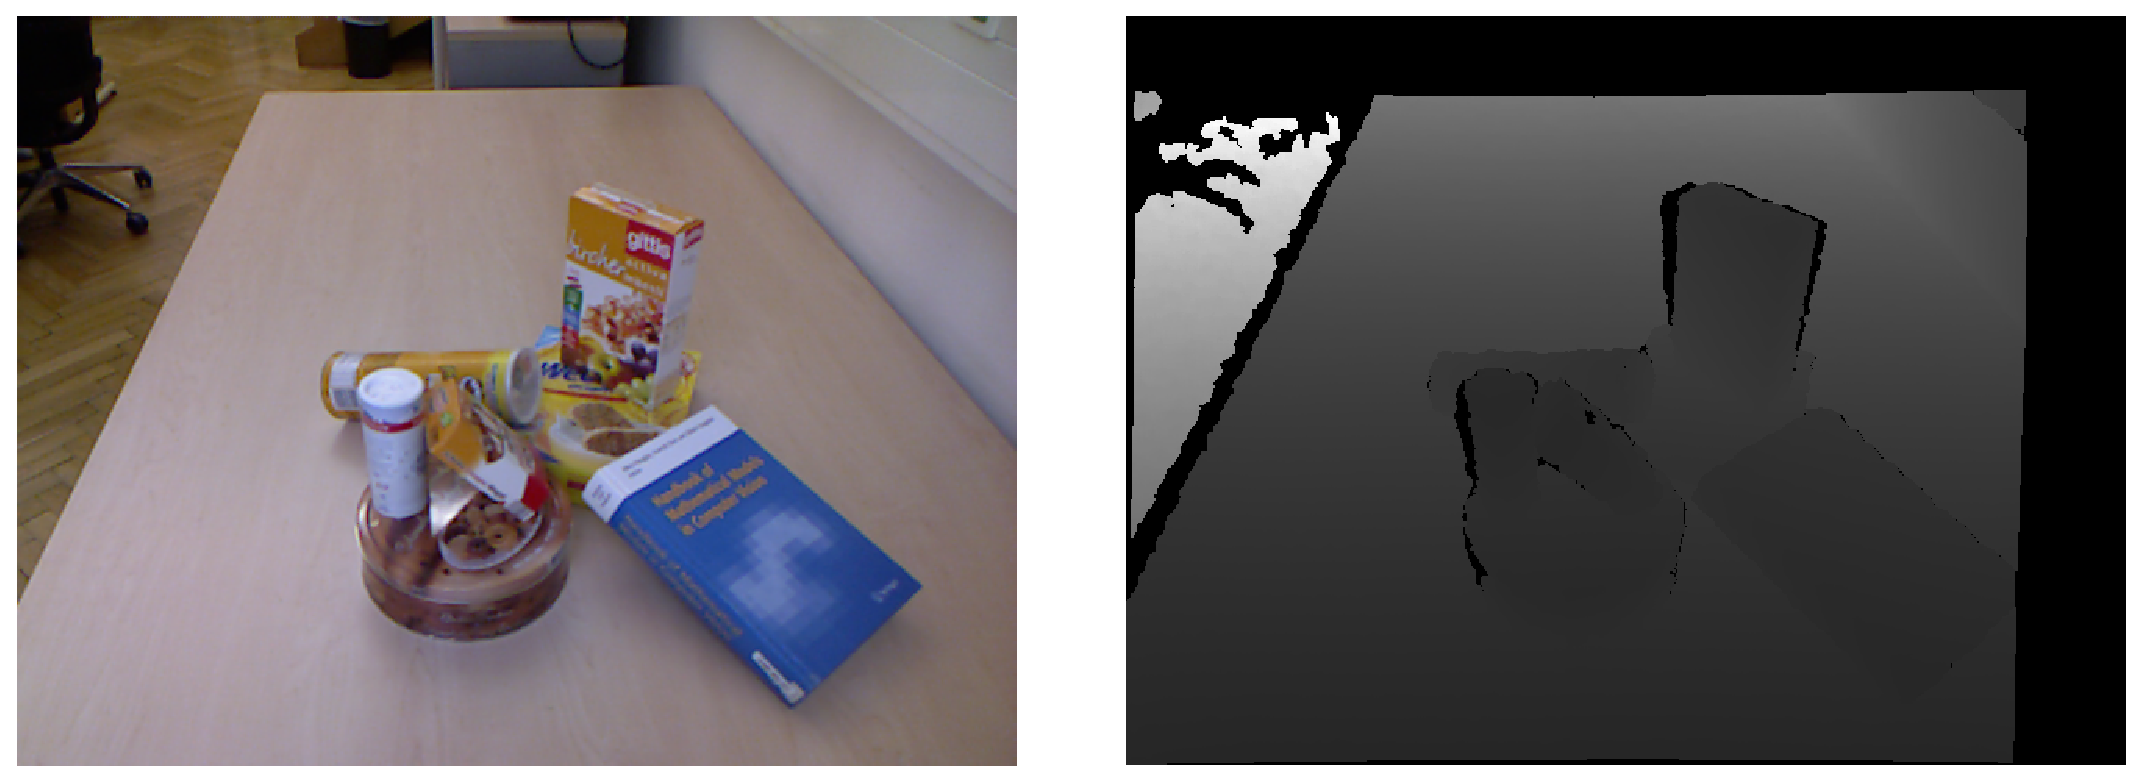
\includegraphics[width=0.8\textwidth]{test.eps}
\caption{The rgb-d image pair used for test.}
\label{fig1}
\end{figure}

Applying bilateral filtering on the depth image with parameters $window\_size=10$, $\sigma_s=2$, and $\sigma_r=20$, we can smooth the depth image while preserving its sharp edges. Figure 2 shows the results.

\begin{figure}[ht]%
\centering
\subfloat[]{{
\includegraphics[width=0.25\linewidth]{fig1.eps}}}%
\qquad
\subfloat[]{{
\includegraphics[width=0.25\linewidth]{fig2.eps}}}%
\caption{Results of bilateral filtering. White points show the original depth, red points show the depth after bilateral filtering.}%
\label{fig2}%
\end{figure}

Applying simple cross bilateral filtering with rgb image is not as effective as bilateral filtering only on the depth image, Figure 3 shows the results. This is because the low correlation between color intensity and depth. We cannot deny the potential of using the color image to improve the quality of depth image, but from this experiment we can see more sophisticated method is needed to achieve this goal.

\begin{figure}[!t]%
\centering
\subfloat[]{{
\includegraphics[width=0.25\linewidth]{fig3.eps}}}%
\qquad
\subfloat[]{{
\includegraphics[width=0.25\linewidth]{fig4.eps}}}%
\caption{Results of cross bilateral filtering. $window\_size=10$, $\sigma_s=2$. For the left image $\sigma_r=6$, for the right image $\sigma_r=0.6$.}%
\label{fig3}%
\end{figure}
\section{References}
\small{
[1] C. Tomasi and R. Manduchi, Bilateral Filtering for Gray and Color Images, \textit{ICCV} 1998.

\noindent [2] G. Petschnigg, M. Agrawala, H. Hoppe, R. Szeliski, M. Cohen, and K. Toyama, Digital Photography with Flash and No-Flash Image Pairs, \textit{SIGGRAPH} 2004.
}
\end{document}